\begin{figure*}
    \centering
    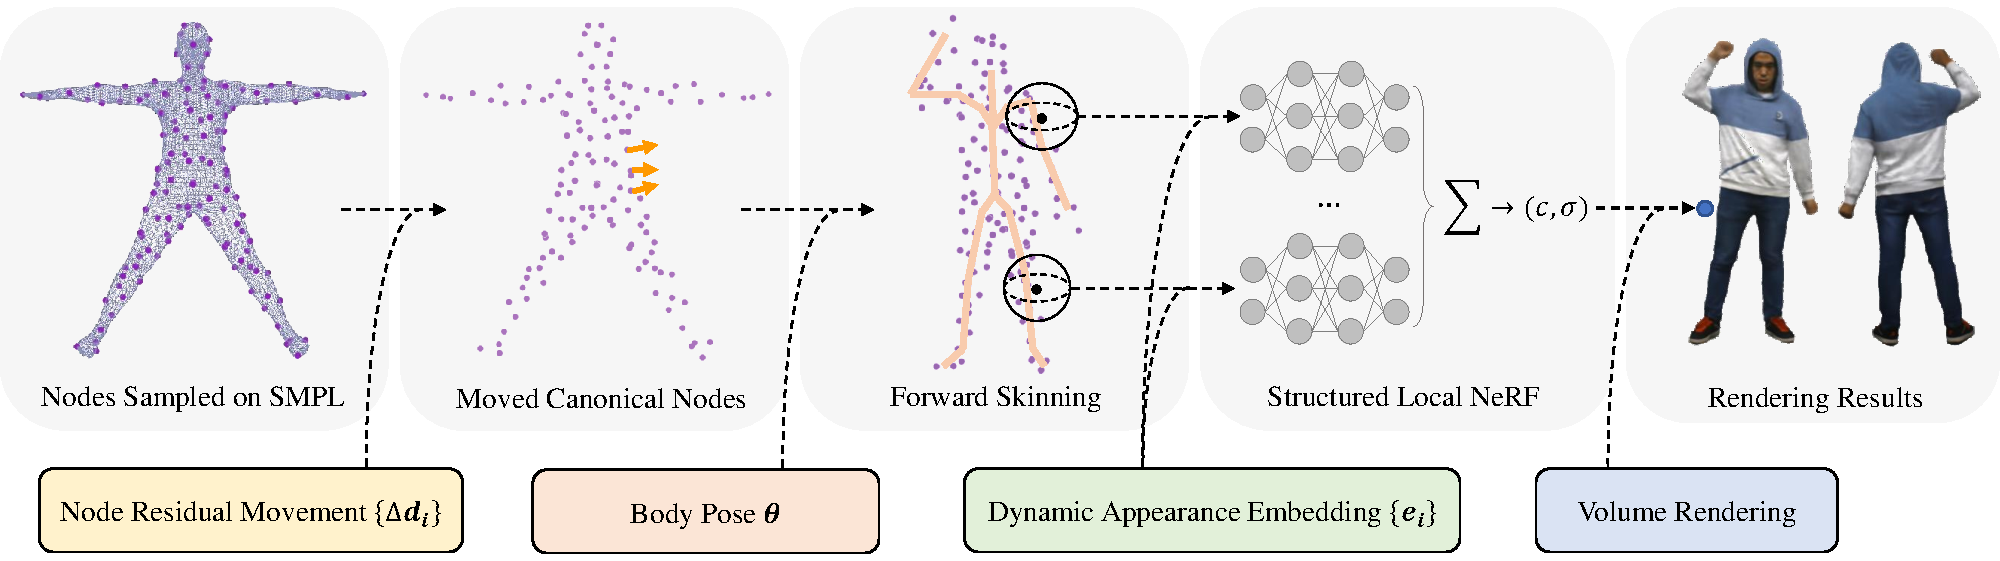
\includegraphics[width=1.0\linewidth]{reprez}
    % \caption{\textbf{Illustration of our clothed human representation.} In our proposed method, we use structured local radiance fields to represent the dynamic appearance of a clothed human character, and model the garment deformation in a coarse-to-fine manner with three set of variables, including body poses as the coarest level, node residual translation as the middle level and dynamic detail embeddings of the local radiance fields as the finest level. }
    \caption{\textbf{Illustration of our clothed human representation.} In our proposed method, we represent the dynamic appearance of a clothed human character using structured local radiance fields attached to pre-defined nodes on the SMPL model. The garment deformations are then modeled in a coarse-to-fine manner with three set of variables, including the body poses as the coarsest level, the node residual translations as the middle level and the dynamic detail embeddings of the local radiance fields as the finest level. }
    \label{fig:reprez}
\end{figure*}


\section{Related Work}
\label{sec:related}

\textbf{Image-based 3D Human Reconstruction.} 
Three-dimensional human character reconstruction is traditionally the very first step towards human avatar modeling. Previous studies focused on using multi-view images~\cite{StarckCGA07,liu2009point,WuShadingHuman,WaschbuschWCSG05,VlasicPBDPRM09} or RGB(D) image sequences~\cite{alldieck2018videoavatar,alldieck2018videoavatar_detailed,yu2017BodyFusion,yu2018doublefusion,Zheng2018HybridFusion,bogo2015detailed,dou2016fusion4d,Motion2Fusion,yu2021function4d,Xiang2020MonoClothCap,habermann2019livecap,Xu2020UnstructuredFusion,guo2017real} for human model reconstruction. Extremely high-quality reconstruction results have also been demonstrated with tens or even hundreds of cameras~\cite{collet2015high}. In order to reduce the difficulty in system setup, human model reconstruction from sparse camera views has been investigated by using neural networks for learning silhouette cues~\cite{MinimalCam18,natsume2019siclope} and stereo cues~\cite{SparseViewHaoLi18}. More recently, various approaches were proposed to reconstruct a 3D human model from a single-view RGB images~\cite{saito2019pifu,saito2020pifuhd,zheng2020pamir,gabeur2019moulding,wang2020normalgan,zhu2019hmd,alldieck2019tex2shape,ARCH2020,He2021archplusplus}. For example, PIFu~\cite{saito2019pifu} and PIFuHD~\cite{saito2020pifuhd} proposed to regress a deep implicit function using pixel-aligned image features and is able to reconstruct high-resolution results. ARCH~\cite{ARCH2020} and ARCH++~\cite{He2021archplusplus} proposed to reconstruct the 3D human model in a canonical pose in order to support animation. Although demonstrating plausible results, these methods rely on large scale dataset of 3D human scans to train the model, and suffer from reconstruction errors and weak generalization capability. In contrast, our method bypasses the reconstruction step and directly learns an animatable avatar from RGB videos. 


\textbf{Neural Scene Representations and Rendering.} 
Representing objects or scenes implicitly with neural networks, is becoming more and more popular for its compactness and strong representation power. Pioneer studies proposed to learn an implicit function where the shapes are embedded into the iso-surface of network output~\cite{park2019deepsdf,chen2019implicit,Occupancy_Networks,zheng2021dit,Genova2020Local,Bozic2021NeuralDeformationGraph,deng2019NASA}. Another line of work on implicit representation aimed at learning scene representations for novel view synthesis from posed 2D images. They represent static scenes using voxel grids of high-dimensional features~\cite{sitzmann2019deepvoxels}, continuous learnable function~\cite{sitzmann2019srns} or neural radiance fields (NeRF)~\cite{mildenhall2020nerf}. NeRF, in particular, shows strong capability of modeling view-dependent effects and thus attracts much attention~\cite{liu2020nsvf,MartinBrualla20arxiv_nerfw,Zhang20arxiv_nerf++,reiser2021kilonerf,yu2021plenoctrees,Garbin21arxiv_FastNeRF,Lombardi2021MVP}. It is later extended for dynamic scenes through deformation learning~\cite{Park20arxiv_nerfies,Pumarola20arxiv_D_NeRF,Gafni20arxiv_DNRF,Tretschk20arxiv_NR-NeRF,Li20arxiv_nsff,Xian20arxiv_stnif,Gao-freeviewvideo,li2021neural3dvideo,shao2022doublefield}. Human motions are usually much more challenging to learn using neural networks, and several works~\cite{peng2021neuralbody,noguchi2021narf,kwon2021neural} incorporated prior from a statistical body template to tackle this difficulty. Note that most of these works can only playback the dynamic sequence that the networks are trained on, while our work aims at animation, which is a much harder task because the method has to generalize to new poses.


\textbf{Animatable Human Avatars.} 
In the last decade, many efforts have been made for achieving expressive and animatable 3D models for human avatars. To facilitate geometric learning, several statistical parametric templates are developed for face~\cite{FLAME:SiggraphAsia2017}, hands~\cite{Romero2017MANO,Moon_2020_ECCV_DeepHandMesh} and minimally clothed body~\cite{loper2015smpl,STAR:2020,SMPL-X:2019,TotalCapture2018}. 
To acquire animatable characters wearing casual clothes, traditional pipelines mostly reconstruct a subject-specific mesh template in advance, and then generate its motions using physics simulation~\cite{Stoll2010Videobased,DRAPE2012}, deformation space modeling~\cite{TotalCapture2018}, or deep learning~\cite{habermann2021realtimeDDC,timur2021driving_signal,Xiang2021ModelingClothing}. The reliance on pre-scanning efforts can be eliminated via deforming a general body template, and several works proposed to directly learn this deformation from geometric data~\cite{CAPE:CVPR:20,pons2017clothcap,Ma:SCALE:2021,Ma:POP:2021} or RGB videos~\cite{alldieck2018videoavatar,alldieck2018videoavatar_detailed,alldieck2019tex2shape,alldieck19octopus}. The texture map and the rasterization step in those methods are later replaced with neural texture maps and image decoders in order to achieve photo-realistic rendering~\cite{Liu2018Neural,liu2020NeuralHumanRendering,Shysheya2019TNR,raj2020anr}. Recently, neural scene representations and rendering techniques are adopted for higher-fidelity results \cite{peng2021animatable_nerf,peng2021neuralbody,neural_actors}. However, state-of-the-art methods only demonstrate results of tightly-fitting garments, while our method is more general in terms of clothes topology and deformation. 
